% !TEX program = pdflatex
\documentclass[11pt, a4paper]{article}

\usepackage[T1]{fontenc}
\usepackage[utf8]{inputenc}
\usepackage{mathpazo}
\usepackage{amsmath, amssymb, amsthm}
\usepackage{mathtools}
\usepackage{geometry}
\usepackage{microtype}
\usepackage{hyperref}
\usepackage{setspace}
\usepackage{titlesec}
\usepackage{abstract}
\usepackage{tikz}
\usetikzlibrary{arrows.meta, positioning, calc}
\usepackage{enumitem}
\usepackage{booktabs}
\usepackage{xcolor}

\geometry{
  top=1.25in, bottom=1.25in,
  left=1.25in, right=1.25in
}

\onehalfspacing

\hypersetup{
  colorlinks=true,
  linkcolor=black,
  citecolor=black,
  urlcolor=black
}

\titleformat{\section}{\large\bfseries}{\thesection.}{0.75em}{}
\titleformat{\subsection}{\normalsize\bfseries}{\thesubsection.}{0.75em}{}
\titleformat{\subsubsection}{\normalsize\itshape}{\thesubsubsection.}{0.75em}{}

\theoremstyle{plain}
\newtheorem{theorem}{Theorem}[section]
\newtheorem{proposition}[theorem]{Proposition}
\newtheorem{lemma}[theorem]{Lemma}
\newtheorem{corollary}[theorem]{Corollary}
\theoremstyle{definition}
\newtheorem{definition}[theorem]{Definition}
\newtheorem{example}[theorem]{Example}
\theoremstyle{remark}
\newtheorem{remark}[theorem]{Remark}
\newtheorem{conjecture}[theorem]{Conjecture}

%% Operators and shorthands
\newcommand{\E}{\mathbb{E}}
\newcommand{\R}{\mathbb{R}}
\newcommand{\N}{\mathbb{N}}
\newcommand{\calX}{\mathcal{X}}
\newcommand{\calY}{\mathcal{Y}}
\newcommand{\calM}{\mathcal{M}}
\newcommand{\calF}{\mathcal{F}}
\newcommand{\calP}{\mathcal{P}}
\newcommand{\calL}{\mathcal{L}}
\newcommand{\calU}{\mathcal{U}}
\newcommand{\calR}{\mathcal{R}}
\newcommand{\simA}{\sim_{\!A}}
\newcommand{\simO}{\sim_{\!O}}
\newcommand{\RHP}{\mathcal{R}_{H}^{\Pi}}
\newcommand{\DA}{D_{A}(\varphi)}
\newcommand{\XmodA}{\calX/{\simA}}
\newcommand{\Adm}{\mathbf{Adm}}
\newcommand{\Set}{\mathbf{Set}}
\newcommand{\Comp}{\mathbf{Comp}}
\newcommand{\op}{\mathrm{op}}
\newcommand{\ob}{\mathrm{ob}}
\newcommand{\Hom}{\mathrm{Hom}}
\newcommand{\id}{\mathrm{id}}
\newcommand{\colim}{\operatorname{colim}}
\newcommand{\Def}{\mathrm{Def}}
\newcommand{\im}{\mathrm{im}}
\DeclareMathOperator{\diam}{diam}

\title{%
  \textbf{The Geometry of Admissibility}\\[0.5em]
  {\large\itshape Quotients, Lattices, Sheaves, and Functorial Reachability}%
}

\author{Flyxion\\[0.4em]
\small Independent Researcher}

\date{June 2026}

\begin{document}
\maketitle

\begin{abstract}
\noindent
A representation of a state space is \emph{admissible} for planning if it
does not collapse states with different reachable futures. This condition
generates a rich mathematical structure that has not been developed in full.
The present paper does so. We begin with a self-contained treatment of
admissibility structures: the reachability equivalence relation $\simA$, the
admissibility quotient $\XmodA$, and the admissibility distortion $D_A(\varphi)$
measuring departure from the quotient that planning requires. From these
primitive notions we build four interlocking geometric objects. First, the
\emph{category} $\Adm$ of admissibility structures, in which admissible
representations are exactly the morphisms and the admissibility quotient
$q_A\colon \calX \to \XmodA$ is the initial object in the subcategory of
admissible projections---a universal property that is strictly stronger than
calling $q_A$ the ``largest safe equivalence relation.'' Second, the
\emph{quotient lattice} $\calL(\calX)$ of equivalence relations on $\calX$
ordered by coarseness, on which admissibility distortion is a monotone height
function and every compression morphism is a step toward higher distortion;
the compression--admissibility tradeoff is a functor from the category of
encoders to the poset of non-negative reals. Third, the \emph{reachability
sheaf} $\calF_A$ over the Alexandrov topology $\tau_A$ generated by reachability
sets: its global sections are exactly the planning-adequate representations,
while the observation presheaf $\calF_O$ over the coarser observation topology
$\tau_O$ yields only local sections; the impossibility of assembling local
observational data into a complete reachability description is a failure of the
sheaf gluing condition, and we propose it as the geometric form of the
Observational--Interventional Separation Theorem. Fourth, \emph{temporal
admissibility functors} $\mathbf{X}\colon \mathbf{T} \to \Adm$ representing
evolving state spaces: meta-admissibility---the requirement that
self-modifications preserve reachability structure---is equivalent to the
functor condition, and comparisons between developmental trajectories are
natural transformations. We conclude with a precise conjecture relating
admissibility distortion to the first \v{C}ech cohomology of the reachability
sheaf, and with an open problems section surveying the cohomological,
topos-theoretic, and persistent-homological directions that the framework opens.
\end{abstract}

\newpage

\tableofcontents

\newpage

%% =====================================================================
\section{Introduction}
\label{sec:intro}
%% =====================================================================

Planning in a learned state space requires the representation to preserve a
specific kind of information: it must not identify states that differ in which
futures are reachable under the available policies. A representation satisfying
this condition is called \emph{admissible}. One that violates it incurs
\emph{admissibility distortion}: it conflates states that are behaviourally
distinct, causing plans constructed in the representation space to fail when
executed in the environment.

The admissibility condition is a natural object of study independently of its
motivating context. It defines an equivalence relation on state spaces, an
induced quotient, a notion of morphism between structured spaces, a partial
order on representations, and a quantitative functional measuring deviation
from the ideal. Each of these objects belongs to a classical mathematical
tradition---category theory, lattice theory, sheaf theory---and each
connection yields results that would be invisible from the planning-theoretic
perspective alone.

The purpose of this paper is to develop these connections systematically. The
paper is entirely self-contained: all notions from the admissibility programme
are defined from scratch, and the main results are proved in full without
external reference. The mathematical prerequisites are basic category theory
at the level of the standard graduate texts on the subject and elementary
sheaf theory; both are recalled where needed. No background in reinforcement
learning or representation learning is assumed.

The paper is organised as follows. Section~\ref{sec:foundations} develops
the admissibility framework from primitive notions: state spaces, policy
classes, reachability, the admissibility equivalence relation, the quotient,
and distortion. Section~\ref{sec:cat} constructs the category $\Adm$ of
admissibility structures and proves the universal property of the admissibility
quotient. Section~\ref{sec:lattice} develops the quotient-lattice structure
and the compression--admissibility tradeoff as a functor.
Section~\ref{sec:sheaf} constructs the reachability sheaf over the Alexandrov
topology, defines the observation presheaf, and proves the sheaf formulation
of the Observational--Interventional Separation Theorem.
Section~\ref{sec:cohomology} proposes the cohomological interpretation of
admissibility distortion and states the central open conjecture.
Section~\ref{sec:temporal} treats evolving state spaces via temporal
admissibility functors and characterises meta-admissibility as a functor
condition. Section~\ref{sec:synthesis} assembles the four structures into a
unified geometric picture. Section~\ref{sec:open} surveys open problems.

\medskip
\noindent\textbf{Notation.} Throughout, $\calX$ denotes a state space (a set),
$\calM$ a representation space, $\Pi$ a policy class, $H \in \N$ a planning
horizon, $\calP(\calX)$ the power set of $\calX$, and $(\R_{\geq 0}, \leq)$
the poset of non-negative reals. Category-theoretic notation follows standard
usage: objects, morphisms, composition $\circ$, identity $\id$.

\medskip
\noindent\textbf{Motivating example: small-object detection.}
The admissibility condition appears concretely in visual inspection systems.
In industrial fault detection, small defects---cracked insulators, loose
bolts---may occupy regions of an image that are statistically nearly
indistinguishable from background texture after standard compression and
pooling operations. Yet their reachable operational futures differ dramatically:
one leads to continued safe operation, the other to equipment failure. Standard
convolutional encoders, optimised for reconstruction or classification accuracy,
may collapse these visually similar regions into identical or nearby
representation codes. Recent architectures for small-object detection address
this by explicitly augmenting the encoder with edge-sensitive features and
multi-scale context, reintroducing precisely the distinctions that would
otherwise be lost. From the admissibility geometry perspective, the
admissibility-critical states occupy a low-measure but high-consequence region
of the quotient lattice: they lie just above the admissibility threshold
$\simA$, and any compression that passes through this boundary incurs
positive admissibility distortion. The architectural interventions can be
understood as admissibility-preserving design choices that prevent the
encoder from crossing this boundary.

%% =====================================================================
\section{Foundations: Admissibility Structures}
\label{sec:foundations}
%% =====================================================================

\subsection{State spaces and reachability}

\begin{definition}[State Space and Policy Class]
\label{def:state_space}
A \emph{state space} is a set $\calX$. A \emph{policy class} $\Pi$ is a
collection of functions $\pi\colon \calX \to \Delta(\calX)$, where
$\Delta(\calX)$ denotes the set of probability distributions over $\calX$.
Each $\pi \in \Pi$ is a \emph{policy}: a map from states to distributions over
successor states.
\end{definition}

\begin{definition}[Reachability Set]
\label{def:reach}
Let $H \in \N$, $\Pi$ a policy class. The \emph{$H$-step reachability set}
of a state $x \in \calX$ under $\Pi$ is
\[
  \RHP(x) \;=\; \bigl\{x' \in \calX \;\big|\;
    \exists\,\pi \in \Pi,\;\exists\,\text{path }
    x = x_0, x_1, \ldots, x_H = x' \text{ with }
    x_{t+1} \in \mathrm{supp}(\pi(x_t))\;\forall t\bigr\}.
\]
We sometimes write $\calR(x)$ when $H$ and $\Pi$ are fixed.
\end{definition}

The reachability set $\RHP(x)$ is the set of states that can be reached from
$x$ in exactly $H$ steps by some policy in $\Pi$. Two states are
\emph{behaviourally distinct} at horizon $H$ if they differ in which states
they can reach.

\subsection{The admissibility equivalence relation}

\begin{definition}[Admissibility Equivalence]
\label{def:admissibility_eq}
The \emph{admissibility equivalence relation} $\simA$ on $\calX$ is defined by
\[
  x_1 \simA x_2 \;\iff\; \RHP(x_1) = \RHP(x_2).
\]
The equivalence class of $x$ under $\simA$ is denoted $[x]_A$.
\end{definition}

\begin{lemma}
$\simA$ is an equivalence relation on $\calX$.
\end{lemma}

\begin{proof}
Reflexivity: $\RHP(x) = \RHP(x)$. Symmetry: if $\RHP(x_1) = \RHP(x_2)$
then $\RHP(x_2) = \RHP(x_1)$. Transitivity: if $\RHP(x_1) = \RHP(x_2)$
and $\RHP(x_2) = \RHP(x_3)$ then $\RHP(x_1) = \RHP(x_3)$.
\end{proof}

\subsection{Admissible representations and distortion}

\begin{definition}[Admissible Representation]
\label{def:admissible_rep}
A function $\varphi\colon \calX \to \calM$ is an \emph{admissible
representation} (or \emph{admissible encoder}) if
\[
  \varphi(x_1) = \varphi(x_2) \;\Longrightarrow\; x_1 \simA x_2,
\]
i.e., $\varphi$ does not merge states with different reachable futures.
Equivalently, $x_1 \not\simA x_2 \Rightarrow \varphi(x_1) \neq \varphi(x_2)$:
admissibility-inequivalent states receive distinct codes.
\end{definition}

\begin{remark}
Admissibility is an injectivity condition relative to the admissibility
equivalence classes: $\varphi$ must be injective on the set of equivalence
classes $\XmodA$. It does not require $\varphi$ to be injective on $\calX$
itself; it may merge admissibility-equivalent states.
\end{remark}

The \emph{morphism defect} of an arbitrary (possibly inadmissible) encoder
$\varphi$ is the set of pairs that $\varphi$ collapses but $\simA$ does not:
\[
  \Def(\varphi) \;=\;
  \bigl\{(x_1, x_2) \in \calX \times \calX \;\big|\;
    \varphi(x_1) = \varphi(x_2),\; x_1 \not\simA x_2\bigr\}.
\]
$\varphi$ is admissible if and only if $\Def(\varphi) = \emptyset$.

\begin{definition}[Admissibility Distortion]
\label{def:distortion}
Let $d\colon \calP(\calX) \times \calP(\calX) \to \R_{\geq 0}$ be a
pseudometric on subsets of $\calX$ (for example, the symmetric difference
pseudometric or the Hausdorff metric). The \emph{admissibility distortion}
of $\varphi$ is
\[
  \DA \;=\;
  \E_{(x_1, x_2) \sim \mu}\!\bigl[
    \mathbf{1}[\varphi(x_1) = \varphi(x_2)] \cdot
    d(\RHP(x_1),\, \RHP(x_2))
  \bigr],
\]
where $\mu$ is a distribution on $\calX \times \calX$. The expectation sums
the reachability separation over collapsed pairs.
\end{definition}

\begin{proposition}[Zero-Distortion Characterisation]
\label{prop:zero_dist}
$\DA = 0$ if and only if $\Def(\varphi) = \emptyset$ almost surely under
$\mu$, i.e., if and only if $\varphi$ is admissible $\mu$-almost surely.
\end{proposition}

\begin{proof}
Since $d$ is a pseudometric, $d(\RHP(x_1), \RHP(x_2)) = 0$ iff
$\RHP(x_1) = \RHP(x_2)$ iff $x_1 \simA x_2$. The integrand
$\mathbf{1}[\varphi(x_1) = \varphi(x_2)] \cdot d(\RHP(x_1), \RHP(x_2))$
is non-negative and vanishes on a pair $(x_1, x_2)$ iff either
$\varphi(x_1) \neq \varphi(x_2)$ (the pair is not collapsed) or
$x_1 \simA x_2$ (the collapsed pair is admissibility-equivalent). Hence
the integral vanishes iff there are no collapsed, admissibility-inequivalent
pairs $\mu$-almost surely.
\end{proof}

\subsection{The admissibility quotient}

\begin{definition}[Admissibility Quotient]
\label{def:quotient}
The \emph{admissibility quotient} is the quotient set
$\XmodA = \calX/{\simA}$ together with the canonical surjection
$q_A\colon \calX \to \XmodA$, $q_A(x) = [x]_A$.
\end{definition}

The admissibility quotient is the ``most compressed'' admissible representation
of $\calX$: it merges exactly the pairs that admissibility permits merging,
and no others. This informal description will be given precise content by the
universal property in Section~\ref{sec:cat}.

\begin{example}[Finite Grid]
\label{ex:grid}
Let $\calX = \{1, \ldots, n\}^2$ be a grid world, $\Pi$ the class of
deterministic policies, $H = 1$. States $x_1$ and $x_2$ are admissibility-equivalent
iff their sets of adjacent cells coincide. Interior states with the same
neighbourhood pattern are equivalent; corner and edge states with distinct
adjacency structures are inequivalent. The admissibility quotient identifies
states by their local connectivity type.
\end{example}

\begin{example}[Observation-Equivalent but Reachability-Distinct States]
\label{ex:oist}
Let $\calX = \{s_0^0, s_0^1, s_{\mathrm{safe}}, s_{\mathrm{danger}}\}$. Both
$s_0^0$ and $s_0^1$ have identical passive observation distributions---they are
\emph{observationally equivalent}---but $\RHP(s_0^0) = \{s_{\mathrm{safe}}\}$
and $\RHP(s_0^1) = \{s_{\mathrm{danger}}\}$. Hence $s_0^0 \not\simA s_0^1$
despite their observational indistinguishability. Any admissible encoder must
assign them distinct codes. This is the canonical minimal instance of the
Observational--Interventional Separation phenomenon, developed at length in
Section~\ref{sec:sheaf}.
\end{example}

%% =====================================================================
\section{The Category of Admissibility Structures}
\label{sec:cat}
%% =====================================================================

\subsection{Objects and morphisms}

\begin{definition}[Admissibility Structure]
\label{def:struct}
An \emph{admissibility structure} is a pair $(\calX, \simA)$ where $\calX$
is a set and $\simA$ is the admissibility equivalence relation on $\calX$
generated by a reachability map $x \mapsto \RHP(x)$ as in
Definition~\ref{def:admissibility_eq}. We will sometimes write $(\calX,
\calR)$ to emphasise the reachability map, with $\simA$ understood as the
kernel of $\calR$.
\end{definition}

\begin{definition}[The Category $\Adm$]
\label{def:adm}
The category $\Adm$ has admissibility structures as objects. A
\emph{morphism} $f\colon (\calX, \simA) \to (\calX', \simA')$ is a function
$f\colon \calX \to \calX'$ satisfying the \emph{congruence condition}:
\[
  x_1 \simA x_2 \;\Longrightarrow\; f(x_1) \simA' f(x_2).
\]
Composition is ordinary function composition; the identity morphism on
$(\calX, \simA)$ is $\id_\calX$.
\end{definition}

\begin{lemma}[$\Adm$ is a Category]
\label{lem:category}
$\Adm$ as defined above satisfies the axioms of a category.
\end{lemma}

\begin{proof}
\emph{Identities.} $\id_\calX\colon (\calX, \simA) \to (\calX, \simA)$
satisfies $x_1 \simA x_2 \Rightarrow \id_\calX(x_1) = x_1 \simA x_2 =
\id_\calX(x_2)$, so the congruence condition holds trivially.

\emph{Composition.} If $f\colon (\calX, \simA) \to (\calX', \simA')$ and
$g\colon (\calX', \simA') \to (\calX'', \simA'')$ are morphisms, then
$x_1 \simA x_2 \Rightarrow f(x_1) \simA' f(x_2) \Rightarrow g(f(x_1))
\simA'' g(f(x_2))$, so $g \circ f$ satisfies the congruence condition.

\emph{Unit laws and associativity} follow from the corresponding properties
of function composition.
\end{proof}

\subsection{Admissible representations as morphisms: a precise statement}

The relationship between the admissibility condition of
Definition~\ref{def:admissible_rep} and morphisms in $\Adm$ requires care.
The two conditions are logically distinct: Definition~\ref{def:admissible_rep}
is an injectivity condition (equal codes imply admissibility-equivalent states),
while the morphism condition is a congruence condition (admissibility-equivalent
states have equivalent images). We now show precisely how they are related.

\begin{definition}[Induced Equivalence on the Target]
\label{def:induced_eq}
Given $\varphi\colon \calX \to \calM$, define the equivalence relation
$\simA^\calM$ on $\calM$ by:
\[
  m_1 \simA^\calM m_2 \;\iff\;
  \exists\, x_1, x_2 \in \calX\colon
  \varphi(x_1) = m_1,\; \varphi(x_2) = m_2,\; x_1 \simA x_2.
\]
This is the equivalence relation on $\calM$ generated by identifying image
points of admissibility-equivalent states.
\end{definition}

\begin{proposition}[Admissible Representations and Morphisms]
\label{prop:morph}
Let $\varphi\colon \calX \to \calM$ and let $\simA^\calM$ be the induced
equivalence on $\calM$ as above.

\begin{enumerate}[label=(\roman*),noitemsep]
  \item $\varphi$ is a morphism $(\calX, \simA) \to (\calM, \simA^\calM)$
    in $\Adm$ for any choice of $\varphi$.
  \item $\varphi$ is admissible (Definition~\ref{def:admissible_rep}) if and
    only if $\varphi$ is injective on admissibility classes: the map
    $\bar\varphi\colon \XmodA \to \calM$ given by $\bar\varphi([x]_A) =
    \varphi(x)$ is injective.
  \item If $\varphi$ is admissible, then $\varphi$ is a morphism from
    $(\calX, \simA)$ to $(\calM, \sim_\varphi)$, where $\sim_\varphi$ is
    the kernel equivalence $m_1 \sim_\varphi m_2 \iff m_1 = m_2$
    (the discrete equivalence on $\im(\varphi)$).
\end{enumerate}
\end{proposition}

\begin{proof}
\emph{(i).} If $x_1 \simA x_2$, then by definition $\varphi(x_1) \simA^\calM
\varphi(x_2)$ (taking $x_1, x_2$ as witnesses). So the congruence condition
holds universally.

\emph{(ii).} $\bar\varphi$ is well-defined by any function: $\bar\varphi([x]_A)
= \varphi(x)$ requires checking that if $[x_1]_A = [x_2]_A$ (i.e., $x_1 \simA
x_2$) then $\varphi(x_1) = \varphi(x_2)$. This is exactly the admissibility
condition: $\varphi(x_1) = \varphi(x_2) \Rightarrow x_1 \simA x_2$ is
contraposited to $x_1 \not\simA x_2 \Rightarrow \varphi(x_1) \neq \varphi(x_2)$,
which means the map $[x]_A \mapsto \varphi(x)$ is well-defined and injective.
Conversely, if $\bar\varphi$ is injective and well-defined, then
$\varphi(x_1) = \varphi(x_2)$ implies $\bar\varphi([x_1]_A) =
\bar\varphi([x_2]_A)$, hence $[x_1]_A = [x_2]_A$ by injectivity, hence
$x_1 \simA x_2$.

\emph{(iii).} If $\varphi$ is admissible, then $x_1 \simA x_2 \Rightarrow
\varphi(x_1) = \varphi(x_2)$: admissibility-equivalent states map to identical
codes. Identical codes are trivially equivalent under the discrete equivalence
on $\im(\varphi)$, so the congruence condition is satisfied.
\end{proof}

\begin{remark}
Part~(i) of Proposition~\ref{prop:morph} shows that every function
$\varphi\colon \calX \to \calM$ is a morphism from $(\calX, \simA)$ to
$(\calM, \simA^\calM)$ once the target is equipped with the induced equivalence.
The interesting content of admissibility is (ii): it characterises when $\varphi$
factors injectively through the admissibility quotient. The morphism condition
in $\Adm$ is a congruence condition, while admissibility is an injectivity
condition; they are equivalent only when the target equivalence is the
discrete one (equal images), which is the case for admissible encoders by (iii).
\end{remark}

\subsection{The universal property of the admissibility quotient}

The universal property of $q_A$ classifies maps that \emph{factor through}
the quotient. A map $\varphi\colon \calX \to \calM$ factors through $q_A$ at
the set level---meaning $\varphi = \bar\varphi \circ q_A$ for some
$\bar\varphi\colon \XmodA \to \calM$---if and only if $\varphi$ is
\emph{constant on admissibility classes}: $x_1 \simA x_2 \Rightarrow
\varphi(x_1) = \varphi(x_2)$. We call such maps \emph{class-constant}.
Admissibility (Definition~\ref{def:admissible_rep}) is a different, dual
condition: a map is admissible iff it is \emph{injective} on admissibility
classes, meaning the induced map $\bar\varphi\colon \XmodA \to \calM$ is
injective. The universal property governs factoring; admissibility governs the
injectivity of the factor.

\begin{theorem}[Universal Property of $q_A$]
\label{thm:universal}
For any class-constant map $\varphi\colon \calX \to \calM$ (i.e., satisfying
$x_1 \simA x_2 \Rightarrow \varphi(x_1) = \varphi(x_2)$), there exists a
unique map $\bar\varphi\colon \XmodA \to \calM$ such that the diagram
\begin{equation}
\label{eq:universal}
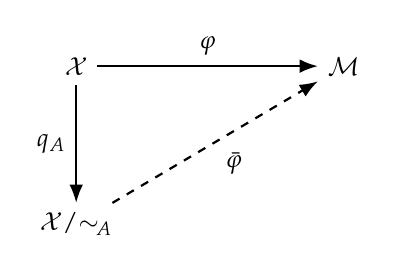
\begin{tikzpicture}[baseline=(current bounding box.center),
  node distance=2.0cm, every node/.style={font=\small}]
  \node (X)  {$\calX$};
  \node (M)  [right=2.8cm of X] {$\calM$};
  \node (Q)  [below=1.5cm of X] {$\XmodA$};
  \draw[-Latex,thick] (X) -- node[above]{$\varphi$} (M);
  \draw[-Latex,thick] (X) -- node[left]{$q_A$} (Q);
  \draw[-Latex,dashed,thick] (Q) -- node[below right]{$\bar\varphi$} (M);
\end{tikzpicture}
\end{equation}
commutes: $\varphi = \bar\varphi \circ q_A$. Moreover, $\bar\varphi$ is a
morphism $(\XmodA, \simA^*) \to (\calM, \simA^\calM)$ in $\Adm$, where
$\simA^*$ is the equivalence on $\XmodA$ defined by $[x_1]_A \simA^*
[x_2]_A \iff x_1 \simA x_2$, and $\simA^\calM$ is the induced equivalence
of Definition~\ref{def:induced_eq}.
\end{theorem}

\begin{proof}
\emph{Well-definedness.} Define $\bar\varphi([x]_A) = \varphi(x)$. If
$[x_1]_A = [x_2]_A$ then $x_1 \simA x_2$, hence $\varphi(x_1) = \varphi(x_2)$
by class-constancy of $\varphi$, so $\bar\varphi$ is well-defined.

\emph{Commutativity.} $\bar\varphi(q_A(x)) = \bar\varphi([x]_A) = \varphi(x)$.

\emph{Uniqueness.} Any $\psi\colon \XmodA \to \calM$ with $\psi \circ q_A =
\varphi$ must satisfy $\psi([x]_A) = \varphi(x)$ for all $x$, since every
element of $\XmodA$ is $[x]_A$ for some $x$. Hence $\psi = \bar\varphi$.

\emph{Morphism condition.} If $[x_1]_A \simA^* [x_2]_A$ in $\XmodA$, then
$x_1 \simA x_2$, so by definition $\varphi(x_1) \simA^\calM \varphi(x_2)$,
i.e., $\bar\varphi([x_1]_A) \simA^\calM \bar\varphi([x_2]_A)$.
\end{proof}

\begin{proposition}[Admissibility as Injectivity of the Factor]
\label{prop:admissible_factor}
Let $\varphi\colon \calX \to \calM$ be class-constant, and let
$\bar\varphi\colon \XmodA \to \calM$ be the unique factor of
Theorem~\ref{thm:universal}. Then $\varphi$ is admissible
(Definition~\ref{def:admissible_rep}) if and only if $\bar\varphi$ is
injective.
\end{proposition}

\begin{proof}
$\bar\varphi$ injective means: $\bar\varphi([x_1]_A) = \bar\varphi([x_2]_A)
\Rightarrow [x_1]_A = [x_2]_A$, i.e., $\varphi(x_1) = \varphi(x_2) \Rightarrow
x_1 \simA x_2$. This is exactly Definition~\ref{def:admissible_rep}.
\end{proof}

The correct categorical picture is therefore:
\[
  \calX \;\xrightarrow{\;q_A\;}\; \XmodA \;\xrightarrow{\;\bar\varphi\;}\; \calM,
\]
where $q_A$ is the universal quotient map, $\bar\varphi$ is the unique
factor (existing for all class-constant $\varphi$), and admissibility is
precisely the condition that $\bar\varphi$ is injective. The admissibility
quotient $q_A$ is not merely the ``largest safe equivalence relation''; it is
the object through which every class-constant representation factors, and
admissible representations are those for which this factoring is injective.

\begin{corollary}[Initiality of $q_A$]
\label{cor:initial}
In the full subcategory $\Adm_{\calX}$ of $\Adm$ whose objects are class-constant
and admissible maps from $\calX$ (i.e., maps $\varphi\colon \calX \to \calM$
satisfying $x_1 \simA x_2 \iff \varphi(x_1) = \varphi(x_2)$), the canonical
quotient map $q_A\colon \calX \to \XmodA$ is initial: there is a unique
morphism from $q_A$ to every other object.
\end{corollary}

\begin{proof}
For any object $\varphi\colon \calX \to \calM$ in $\Adm_\calX$, the condition
$x_1 \simA x_2 \iff \varphi(x_1) = \varphi(x_2)$ ensures class-constancy.
Theorem~\ref{thm:universal} gives a unique $\bar\varphi\colon \XmodA \to \calM$
with $\varphi = \bar\varphi \circ q_A$. By Proposition~\ref{prop:admissible_factor},
$\bar\varphi$ is injective. This $\bar\varphi$ is the unique morphism from
$q_A$ to $\varphi$ in $\Adm_\calX$.
\end{proof}

\subsection{The morphism defect as a measure of non-initiality}

For an inadmissible encoder $\varphi$, the morphism defect
$\Def(\varphi) \neq \emptyset$ and $\varphi$ does not factor through $q_A$.
The admissibility distortion $\DA$ quantifies \emph{how far} $\varphi$ is
from being a morphism in $\Adm$:
\[
  \DA = \E_\mu\!\bigl[\mathbf{1}_{\Def(\varphi)}(x_1,x_2) \cdot
    d(\RHP(x_1), \RHP(x_2))\bigr].
\]
This is zero iff $\Def(\varphi) = \emptyset$ a.s., iff $\varphi$ is
(strongly) admissible a.s., iff $\varphi$ factors through $q_A$
(Proposition~\ref{prop:zero_dist}).

%% =====================================================================
\section{The Quotient Lattice and Compression Morphisms}
\label{sec:lattice}
%% =====================================================================

\subsection{The lattice of quotients}

\begin{definition}[Quotient Lattice]
\label{def:quotient_lattice}
For a fixed state space $\calX$, the \emph{quotient lattice}
$\calL(\calX)$ is the set of equivalence relations on $\calX$ ordered by
inclusion:
\[
  {\sim_1} \leq {\sim_2} \;\iff\; {\sim_1} \subseteq {\sim_2}
  \;\iff\; \forall x_1, x_2\colon x_1 \sim_1 x_2 \Rightarrow x_1 \sim_2 x_2.
\]
We say $\sim_2$ is \emph{coarser} than $\sim_1$ (and $\sim_1$ is
\emph{finer} than $\sim_2$) when ${\sim_1} \leq {\sim_2}$.
\end{definition}

\begin{lemma}[$\calL(\calX)$ is a Complete Lattice]
\label{lem:lattice}
$(\calL(\calX), \leq)$ is a complete lattice with meet given by intersection
$\sim_1 \wedge \sim_2 = {\sim_1} \cap {\sim_2}$ and join given by the
equivalence closure of the union $\sim_1 \vee \sim_2 = \overline{{\sim_1}
\cup {\sim_2}}$. The bottom element is the diagonal (equality) relation
$\Delta_\calX$ and the top element is the total relation $\calX \times \calX$.
\end{lemma}

\begin{proof}
Standard result in lattice theory. Intersection of equivalence relations is
an equivalence relation. Equivalence closure of a union of equivalence relations
is the smallest equivalence relation containing both; its existence follows
from the fact that the intersection of any family of equivalence relations is
an equivalence relation, so the closure is the intersection of all equivalence
relations containing the union.
\end{proof}

Every equivalence relation $\sim_\varphi$ on $\calX$ induced by an encoder
$\varphi$ (the kernel: $x_1 \sim_\varphi x_2 \iff \varphi(x_1) = \varphi(x_2)$)
defines a point in $\calL(\calX)$.

\begin{proposition}[Lattice Embedding]
\label{prop:lattice}
The assignment ${\sim} \mapsto \calX/{\sim}$ defines an order-reversing
embedding of $(\calL(\calX), \leq)$ into $\Adm$: if ${\sim_1} \leq {\sim_2}$,
there is a canonical surjective morphism $\pi_{12}\colon (\calX/{\sim_1},
\sim_1^*) \to (\calX/{\sim_2}, \sim_2^*)$ in $\Adm$, and this assignment is
functorial.
\end{proposition}

\begin{proof}
If ${\sim_1} \subseteq {\sim_2}$, then any $\sim_1$-class $[x]_{\sim_1}$
is contained in a unique $\sim_2$-class $[x]_{\sim_2}$. Define
$\pi_{12}([x]_{\sim_1}) = [x]_{\sim_2}$. This is well-defined: if
$[x]_{\sim_1} = [y]_{\sim_1}$ then $x \sim_1 y$, hence $x \sim_2 y$, hence
$[x]_{\sim_2} = [y]_{\sim_2}$. It is surjective since $q_{\sim_2} = \pi_{12}
\circ q_{\sim_1}$. The morphism condition in $\Adm$ holds: $[x]_{\sim_1}
\sim_1^* [y]_{\sim_1}$ in $\calX/{\sim_1}$ means $[x]_{\sim_1} =
[y]_{\sim_1}$, so $\pi_{12}([x]) = \pi_{12}([y])$, and equal elements are
trivially $\sim_2^*$-related. Functoriality ($\pi_{12} = \pi_{23} \circ
\pi_{12}$ when appropriate) follows from transitivity of class containment.
\end{proof}

\subsection{Compression as upward movement}

\begin{definition}[Compression Morphism]
\label{def:compression}
A \emph{compression morphism} from encoder $\varphi_1$ to encoder $\varphi_2$
is the canonical surjection $\pi\colon \calX/{\sim_{\varphi_1}} \to
\calX/{\sim_{\varphi_2}}$ in $\Adm$ whenever ${\sim_{\varphi_1}} \leq
{\sim_{\varphi_2}}$. We say $\varphi_2$ is a \emph{compression} of $\varphi_1$.
\end{definition}

Compression morphisms exist exactly when the second encoder merges at least
as many pairs as the first. In $\calL(\calX)$, passing from $\varphi_1$ to
$\varphi_2$ is upward movement toward coarser equivalence relations.

\begin{theorem}[Monotonicity of Distortion]
\label{thm:monotone}
If ${\sim_{\varphi_1}} \leq {\sim_{\varphi_2}}$ (i.e., a compression morphism
exists from $\varphi_1$ to $\varphi_2$), then
\[
  D_A(\varphi_1) \leq D_A(\varphi_2).
\]
Moreover, the increase is given by the \emph{compression cost identity}:
\[
  D_A(\varphi_2) - D_A(\varphi_1)
  = \E_\mu\!\bigl[\mathbf{1}_\mathcal{N}(x_1,x_2)
    \cdot d(\RHP(x_1), \RHP(x_2))\bigr],
\]
where $\mathcal{N} = {\sim_{\varphi_2}} \setminus {\sim_{\varphi_1}}$
is the set of newly collapsed pairs.
\end{theorem}

\begin{proof}
Since ${\sim_{\varphi_1}} \subseteq {\sim_{\varphi_2}}$, the support of the
indicator $\mathbf{1}[\varphi_1(x_1) = \varphi_1(x_2)]$ is contained in the
support of $\mathbf{1}[\varphi_2(x_1) = \varphi_2(x_2)]$. Write
${\sim_{\varphi_2}} = {\sim_{\varphi_1}} \cup \mathcal{N}$ (disjoint union
over admissibility-inequivalent pairs). Then
\begin{align*}
  D_A(\varphi_2)
  &= \E_\mu\!\bigl[\mathbf{1}_{{\sim_{\varphi_2}}}
      \cdot d(\RHP(x_1), \RHP(x_2))\bigr] \\
  &= \E_\mu\!\bigl[\mathbf{1}_{{\sim_{\varphi_1}}}
      \cdot d(\cdot)\bigr]
    + \E_\mu\!\bigl[\mathbf{1}_\mathcal{N}
      \cdot d(\cdot)\bigr] \\
  &= D_A(\varphi_1) + \E_\mu\!\bigl[\mathbf{1}_\mathcal{N}
      \cdot d(\RHP(x_1), \RHP(x_2))\bigr].
\end{align*}
Since $d \geq 0$, the second term is non-negative, establishing $D_A(\varphi_1)
\leq D_A(\varphi_2)$.
\end{proof}

\begin{remark}[Distortion as a Height Function]
Theorem~\ref{thm:monotone} gives $\DA$ the structure of a height function on
$\calL(\calX)$: it increases weakly as one moves upward toward coarser
equivalence relations. Every compression morphism is a step toward higher
distortion. The admissibility quotient $q_A$ corresponds to the point
$\simA \in \calL(\calX)$, and any encoder above $\simA$ in the lattice
(coarser than $\simA$) collapses admissibility-inequivalent pairs, incurring
positive distortion.
\end{remark}

\subsection{The compression--admissibility tradeoff as a functor}

\begin{definition}[Category of Encoders]
\label{def:comp_cat}
The \emph{category of encoders} $\Comp(\calX)$ has encoders
$\varphi\colon \calX \to \calM$ as objects and compression morphisms as
morphisms. Composition is composition of the canonical surjections.
\end{definition}

\begin{proposition}[Distortion Functor]
\label{prop:distortion_functor}
The admissibility distortion defines a functor
\[
  D_A\colon \Comp(\calX) \;\longrightarrow\; (\R_{\geq 0}, \leq),
\]
where $(\R_{\geq 0}, \leq)$ is the poset regarded as a category (one morphism
$r_1 \to r_2$ whenever $r_1 \leq r_2$). This functor sends compression
morphisms to inequalities $D_A(\varphi_1) \leq D_A(\varphi_2)$.
\end{proposition}

\begin{proof}
Theorem~\ref{thm:monotone} establishes that $D_A$ is order-preserving on the
quotient lattice, hence on $\Comp(\calX)$. Functoriality reduces to this
monotonicity, together with the trivial observation that identity morphisms
map to equality $D_A(\varphi) \leq D_A(\varphi)$.
\end{proof}

The information bottleneck problem asks: given a mutual information budget $I$,
find the most compressed encoder with $D_A(\varphi) \leq \epsilon$. In
$\Comp(\calX)$, this is: find the initial object in the full subcategory of
encoders with distortion at most $\epsilon$. The Lagrangian relaxation
\[
  \min_\varphi \bigl[I(\calX; \varphi(\calX)) + \lambda \cdot D_A(\varphi)\bigr]
\]
traces a path in $\Comp(\calX)$ parameterised by $\lambda \geq 0$: at
$\lambda = 0$ we recover maximal compression (the terminal object, coarsest
encoder), and as $\lambda \to \infty$ the path converges to $q_A$ (the
initial admissible object of Corollary~\ref{cor:initial}).

\begin{example}[Token Pruning as Controlled Quotienting]
\label{ex:token}
Transformer-based vision models operate on sequences of visual tokens. Token
pruning reduces the sequence length by discarding tokens judged uninformative.
Each pruning operation induces an equivalence relation $\sim_{\mathrm{prune}}$
on the token space: tokens collapsed to a single representation become
equivalent under $\sim_{\mathrm{prune}}$. Pruning is therefore movement in
the quotient lattice $\calL(\calX)$: each step coarsens the equivalence
relation. The performance question---does pruning degrade task accuracy?---is
precisely the admissibility question: does the induced compression cross the
threshold $\simA$ for the downstream task?

Architectures that compute per-token importance scores before pruning are
performing an approximation to admissibility-aware quotient construction: they
attempt to preserve the equivalence classes that the task (here, keypoint
localisation or action recognition) requires to remain distinct, and collapse
only those tokens whose reachable ``inference futures'' are indistinguishable.
The compression cost identity of Theorem~\ref{thm:monotone} gives a precise
account of the distortion incurred by each pruning step: it is the expected
reachability separation over the set of newly collapsed token pairs.
\end{example}

%% =====================================================================
\section{The Reachability Sheaf}
\label{sec:sheaf}
%% =====================================================================

\subsection{The Alexandrov topology on $\calX$}

The fixed-horizon reachability relation $x' \in \RHP(x)$ does not in general
define a preorder: reflexivity requires every state to reach itself in exactly
$H$ steps (which fails for $H \geq 1$ in acyclic environments), and transitivity
requires that reachability in $H$ steps followed by reachability in $H$ steps
yields reachability in $H$ steps (which holds only if $H + H = H$, i.e., never).
We therefore base the topology on the \emph{transitive closure} of reachability,
which is the natural planning-relevant notion: a state is accessible if it can
be reached in \emph{some} finite number of steps.

\begin{definition}[Reachability Preorder]
\label{def:reach_preorder}
The \emph{reachability preorder} $\leq_A$ on $\calX$ is defined by
\[
  x' \leq_A x \;\iff\;
  \exists\, h \in \N,\;\exists\,\pi \in \Pi,\;
  \exists\,\text{path } x = x_0, x_1, \ldots, x_h = x'
  \text{ with } x_{t+1} \in \mathrm{supp}(\pi(x_t))\;\forall t,
\]
i.e., $x'$ is at or below $x$ in the order iff $x'$ is reachable from $x$
in some finite number of steps under some policy. We write
$\calR^\Pi(x) = \{x' : x' \leq_A x\}$ for the full reachability set of $x$.
\end{definition}

\begin{remark}[Relation to the Fixed-Horizon Reachability Set]
The distortion functional $\DA$ of Definition~\ref{def:distortion} uses the
fixed-horizon reachability sets $\RHP(x)$ as the objects being compared. The
preorder $\leq_A$ uses the \emph{cumulative} reachability $\calR^\Pi(x) =
\bigcup_{h \geq 0} \mathcal{R}_h^\Pi(x)$. These are the appropriate objects
for two different purposes: the fixed-horizon set captures the precise
planning consequences at horizon $H$ and is the right object for the distortion
functional; the cumulative set captures the long-run accessibility structure
of the state space and is the right basis for a topology. The admissibility
equivalence relation $\simA$ is defined in terms of $\RHP$ and remains
unchanged.
\end{remark}

\begin{lemma}[$\leq_A$ is a Preorder]
\label{lem:preorder}
The relation $\leq_A$ is reflexive and transitive, hence a preorder on $\calX$.
\end{lemma}

\begin{proof}
\emph{Reflexivity.} Every state $x$ reaches itself in $h = 0$ steps (the
empty path), so $x \leq_A x$.

\emph{Transitivity.} If $x'' \leq_A x'$ and $x' \leq_A x$, then there exist
paths of lengths $h_1$ and $h_2$ from $x$ to $x'$ and from $x'$ to $x''$
respectively. Concatenating these paths gives a path of length $h_1 + h_2$
from $x$ to $x''$, so $x'' \leq_A x$.
\end{proof}

\begin{definition}[Reachability Topology]
\label{def:reach_top}
The \emph{reachability topology} $\tau_A$ on $\calX$ is the
\emph{Alexandrov topology} of the preorder $\leq_A$: a set
$U \subseteq \calX$ is open iff it is an \emph{up-set} of $\leq_A$,
\[
  x \in U \text{ and } x' \leq_A x \;\Longrightarrow\; x' \in U,
\]
i.e., if a state is in $U$ then all states reachable from it are also in $U$.
\end{definition}

\begin{lemma}[$\tau_A$ is a Topology]
\label{lem:topology}
The collection $\tau_A$ is a topology on $\calX$.
\end{lemma}

\begin{proof}
$\emptyset$ and $\calX$ satisfy the up-set condition vacuously and trivially.
Arbitrary unions of up-sets are up-sets: if $x \in \bigcup_\alpha U_\alpha$
and $x' \leq_A x$, then $x \in U_\alpha$ for some $\alpha$, so $x' \in
U_\alpha$. Finite intersections of up-sets are up-sets: if $x \in U_1 \cap
\cdots \cap U_n$ and $x' \leq_A x$, then $x' \in U_i$ for each $i$, so
$x' \in U_1 \cap \cdots \cap U_n$.
\end{proof}

\begin{remark}[Basis for $\tau_A$]
The principal up-sets ${\uparrow}x = \{x' \in \calX : x' \leq_A x\} =
\calR^\Pi(x)$ are open in $\tau_A$ (by definition of up-sets) and form a
basis: every open set is a union of principal up-sets. This is the Alexandrov
basis theorem applied to $(\calX, \leq_A)$.
\end{remark}

\begin{definition}[Observation Topology]
\label{def:obs_top}
Define the \emph{observation preorder} $\leq_O$ by $x' \leq_O x$ iff
$P(O_{1:\infty} \mid x') = P(O_{1:\infty} \mid x)$, where $O_{1:\infty}$ is
the passive observation sequence generated from state $x$. The
\emph{observation topology} $\tau_O$ is the Alexandrov topology of $\leq_O$.
\end{definition}

The Observational--Interventional Separation phenomenon (see
Example~\ref{ex:oist}) is equivalent to $\tau_O \neq \tau_A$: the two
topologies are in general distinct. The observation topology is typically
coarser---larger equivalence classes, fewer open sets---since it cannot
distinguish states with identical passive distributions but different
reachability structures.

\subsection{The reachability presheaf and sheaf}

\begin{definition}[Reachability Presheaf]
\label{def:reach_presheaf}
The \emph{reachability presheaf} $\calF_A$ on $(\calX, \tau_A)$ assigns to
each open set $U \in \tau_A$ the set of \emph{reachability sections over $U$}:
\[
  \calF_A(U) = \bigl\{ s\colon U \to \calP(\calX)
    \;\big|\; s(x) \subseteq \RHP(x)\;\text{ for all } x \in U \bigr\}.
\]
For $V \subseteq U$ open, the restriction map $\rho_{UV}\colon \calF_A(U)
\to \calF_A(V)$ sends $s \mapsto s|_V$ (restriction of the function to $V$).
\end{definition}

A \emph{section} of $\calF_A$ over $U$ is an element $s \in \calF_A(U)$: a
function assigning to each state in $U$ a subset of its reachable futures.
The canonical global section is $s^*\colon \calX \to \calP(\calX)$,
$s^*(x) = \RHP(x)$: the complete reachability description.

\begin{lemma}[$\calF_A$ is a Sheaf]
\label{lem:sheaf}
$\calF_A$ satisfies the sheaf axioms on $(\calX, \tau_A)$.
\end{lemma}

\begin{proof}
\emph{Locality.} If $s, t \in \calF_A(U)$ and $s|_{U_i} = t|_{U_i}$ for
all opens $U_i$ in a cover of $U$, then $s(x) = t(x)$ for all $x \in U$
(since every $x$ lies in some $U_i$), so $s = t$.

\emph{Gluing.} Given a cover $\{U_i\}$ of $U$ and compatible sections
$s_i \in \calF_A(U_i)$ (compatible meaning $s_i|_{U_i \cap U_j} =
s_j|_{U_i \cap U_j}$ for all $i, j$), define $s\colon U \to \calP(\calX)$
by $s(x) = s_i(x)$ for any $i$ with $x \in U_i$. Compatibility ensures
this is well-defined. Since $s_i(x) \subseteq \RHP(x)$ for all $i$ and all
$x \in U_i$, we have $s(x) \subseteq \RHP(x)$ for all $x \in U$. Hence
$s \in \calF_A(U)$ and $s|_{U_i} = s_i$.
\end{proof}

\subsection{The observation presheaf}

\begin{definition}[Observation Presheaf]
\label{def:obs_presheaf}
The \emph{observation presheaf} $\calF_O$ on $(\calX, \tau_O)$ assigns to
each open $U \in \tau_O$ the set of observation sections over $U$:
\[
  \calF_O(U) = \bigl\{ f\colon U \to \mathcal{D}
    \;\big|\; f(x) = P(O_{1:\infty} \mid x) \text{ for all } x \in U \bigr\},
\]
where $\mathcal{D}$ is the space of probability distributions over observation
sequences. Restriction maps are restrictions of functions.
\end{definition}

Each section of $\calF_O$ over $U$ is (up to the constraint that $f(x)$ must
equal the observation distribution at $x$) essentially the single function
$x \mapsto P(O_{1:\infty} \mid x)$ restricted to $U$. The presheaf records
what passive observation reveals about each state.

\begin{remark}
The observation presheaf $\calF_O$ is actually a sheaf on $(\calX, \tau_O)$
by the same argument as Lemma~\ref{lem:sheaf}: sections are functions into
$\mathcal{D}$, and functions glue uniquely. However, $\calF_O$ is a sheaf on
$(\calX, \tau_O)$, not on $(\calX, \tau_A)$, because the observation topology
is the natural domain for passive observation data.
\end{remark}

\subsection{The gluing failure and the Observational--Interventional Separation}

The canonical global section of $\calF_A$ encodes the complete reachability
structure. Planning requires this global section. Passive observation provides
local sections of $\calF_O$. The central question is whether these local
observational sections can be assembled to determine the global reachability
section.

\begin{theorem}[Sheaf Formulation of Observational--Interventional Separation]
\label{thm:sheaf_oist}
Let $\mathcal{U} = \{U_i\}$ be a cover of $\calX$ by $\tau_O$-open sets.
There exist compatible local sections $s_i \in \calF_O(U_i)$---satisfying
$s_i|_{U_i \cap U_j} = s_j|_{U_i \cap U_j}$ for all $i, j$---that are
consistent with more than one distinct global section of $\calF_A$. That is,
the global reachability section is not uniquely determined by any complete
system of local observational sections.
\end{theorem}

\begin{proof}
By Example~\ref{ex:oist}, there exist states $x_1 = s_0^0$ and $x_2 = s_0^1$
with $P(O_{1:\infty} \mid x_1) = P(O_{1:\infty} \mid x_2)$ but
$\RHP(x_1) \neq \RHP(x_2)$. Since the observation distributions are equal,
$x_1$ and $x_2$ lie in the same $\tau_O$-equivalence class and hence in the
same element of any $\tau_O$-cover $\mathcal{U}$: there exists $U_{i_0}$
with $\{x_1, x_2\} \subseteq U_{i_0}$.

A local section $s_{i_0} \in \calF_O(U_{i_0})$ assigns $s_{i_0}(x) =
P(O_{1:\infty} \mid x)$ for $x \in U_{i_0}$. Since $x_1$ and $x_2$ have
identical observation distributions, the observational data $s_{i_0}$ is
equally consistent with the reachability assignment $x_1 \mapsto \RHP(x_1),
x_2 \mapsto \RHP(x_2)$ and with the swapped assignment $x_1 \mapsto
\RHP(x_2), x_2 \mapsto \RHP(x_1)$.

Both assignments define valid global sections of $\calF_A$ (since both assign
to each state a subset of its actual reachable futures). The local observational
data does not distinguish between them. Hence compatible local sections of
$\calF_O$ do not uniquely determine the global section of $\calF_A$.
\end{proof}

\begin{remark}
Theorem~\ref{thm:sheaf_oist} reformulates an equivalence-relation statement as
a sheaf statement. The equivalence-relation version says: observational
equivalence and admissibility equivalence are distinct relations. The sheaf
version says: local sections of $\calF_O$ do not satisfy the uniqueness part
of sheaf gluing when regarded as data for $\calF_A$. The sheaf formulation is
geometrically richer: it explains \emph{why} the failure occurs (the cover is
too coarse to separate states that $\calF_A$ must separate) and points toward
the cohomological quantification in Section~\ref{sec:cohomology}.
\end{remark}

\begin{example}[Biological Ageing as Local--Global Sheaf Structure]
\label{ex:ageing}
Medical imaging provides a concrete empirical instance of local sections and
global sections in the sense of Theorem~\ref{thm:sheaf_oist}. Separate
predictors trained on imaging data from individual organs---brain, liver, lung,
heart, spine---each estimate an organ-specific biological age, corresponding
to a local section of an ageing sheaf over the anatomical cover of the body.
A whole-body predictor attempts to integrate these local estimates into a
global biological age, corresponding to a global section. The empirical finding
that local organ ages are individually predictable but do not uniquely determine
the global ageing trajectory is precisely the sheaf-theoretic non-uniqueness
of Theorem~\ref{thm:sheaf_oist}: compatible local sections (organ age
estimates) do not determine a unique global section (whole-body biological age)
because different combinations of organ ages can produce the same observational
signature.

Interventional experiments that modify one organ's apparent age while holding
others fixed further illustrate the distinction between local observational
access and global reachability structure: a local change can alter the global
trajectory, but local observation alone cannot predict by how much. This is
the biological analogue of the planning scenario: the global section of
$\calF_A$ (the reachability structure) is not determined by the local sections
of $\calF_O$ (the passive observations), and the admissibility distortion of
any observation-based predictor measures precisely this gap.
\end{example}

%% =====================================================================
\section{Cohomological Perspectives}
\label{sec:cohomology}
%% =====================================================================

Theorem~\ref{thm:sheaf_oist} identifies a failure of gluing: compatible local
observational sections do not determine a unique global reachability section.
In sheaf cohomology, obstructions to gluing are measured by the first
cohomology group of the relevant sheaf. This section sets up the \v{C}ech
cohomology machinery and states the central conjecture of this paper.

\subsection{The \v{C}ech complex}

Let $\mathcal{U} = \{U_i\}_{i \in I}$ be a $\tau_O$-cover of $\calX$,
and let $\calF_A$ be the reachability sheaf of Section~\ref{sec:sheaf}.
The \v{C}ech complex of $\calF_A$ with respect to $\mathcal{U}$ is
\begin{equation}
\label{eq:cech}
  0 \;\longrightarrow\; \calF_A(\calX)
  \;\xrightarrow{\;\delta^0\;}
  \prod_{i \in I} \calF_A(U_i)
  \;\xrightarrow{\;\delta^1\;}
  \prod_{i < j} \calF_A(U_i \cap U_j)
  \;\longrightarrow\; \cdots
\end{equation}
The coboundary maps are:
\begin{align*}
  \delta^0(s)_i &= s|_{U_i}, \\
  \delta^1(s_i)_{ij} &= s_j|_{U_i \cap U_j} - s_i|_{U_i \cap U_j},
\end{align*}
where the difference in the second line requires $\calF_A$ to take values in
an abelian group (see Remark~\ref{rem:linearisation} below). The first
\v{C}ech cohomology group
\[
  \check{H}^1(\mathcal{U}; \calF_A) = \ker(\delta^1) / \im(\delta^0)
\]
classifies the obstructions to lifting compatible local sections to global sections:
a class $[\{s_{ij}\}] \in \check{H}^1(\mathcal{U}; \calF_A)$ is non-trivial
iff the system of local sections $\{s_i\}$ satisfies compatibility on overlaps
but does not come from a global section.

\begin{remark}[Linearisation]
\label{rem:linearisation}
As defined, $\calF_A(U)$ is a set of functions $U \to \calP(\calX)$, not
an abelian group. To define a \v{C}ech complex with $\R$-valued coboundaries,
one passes to a linearisation: replace $\calF_A(U)$ by a sheaf of real vector
spaces via the map $s \mapsto \mathbf{1}_s$ (indicator function on
$\calX \times \calX$), or by working with a sheaf of signed measures on
$\calP(\calX)$. The appropriate linearisation depends on the metric $d$
used to define admissibility distortion $\DA$. We proceed formally under the
assumption that such a linearisation has been fixed, deferring the detailed
construction to future work.
\end{remark}

\subsection{The central conjecture}

We are now in a position to state the main conjecture of this paper. The
admissibility distortion $\DA$ is a non-negative real number quantifying how
far a given encoder $\varphi$ is from admissibility. The first \v{C}ech
cohomology $\check{H}^1(\mathcal{U}; \calF_A)$ is an algebraic object
measuring the obstruction to gluing. The conjecture asserts that these are
related.

\begin{conjecture}[Cohomological Admissibility Obstruction]
\label{conj:cohomology}
Let $\mathcal{U}$ be the $\tau_O$-cover of $\calX$ by observational
indistinguishability classes. After appropriate linearisation of $\calF_A$
as in Remark~\ref{rem:linearisation}, the first \v{C}ech cohomology group
$\check{H}^1(\mathcal{U}; \calF_A)$ is non-trivial if and only if there
exists an inadmissible encoder $\varphi$ (i.e., $\DA > 0$) consistent with
the observational data provided by $\mathcal{U}$. Moreover, there is a
natural map
\[
  \|\cdot\|\colon \check{H}^1(\mathcal{U}; \calF_A) \;\to\; \R_{\geq 0}
\]
(a norm on the cohomology group with respect to the chosen linearisation)
such that
\[
  \|[\delta s]\| \;\geq\; c \cdot \inf_{\varphi\text{ consistent}} \DA
\]
for some constant $c > 0$ depending only on $\mathcal{U}$ and the metric $d$.
\end{conjecture}

\begin{remark}[What would constitute a proof]
A proof of Conjecture~\ref{conj:cohomology} would require: (a) a precise
linearisation of $\calF_A$ as a sheaf of abelian groups; (b) an explicit
identification of the cohomology class $[\delta s]$ associated to an
inadmissible encoder; (c) a norm on $\check{H}^1$ (or a natural map to $\R$)
compatible with the admissibility distortion; and (d) a lower bound on the
norm in terms of $\DA$. Steps (a) and (b) are formal but non-trivial; steps
(c) and (d) are the substantive mathematical content. We believe this programme
is tractable and constitutes the most important open problem in the geometry
of admissibility.
\end{remark}

\begin{remark}[Relation to the Separation Theorem]
Theorem~\ref{thm:sheaf_oist} establishes the \emph{existence} of a non-trivial
obstruction (there are observational covers that do not determine the global
reachability section). Conjecture~\ref{conj:cohomology} asserts that this
obstruction is \emph{measured} by admissibility distortion via a cohomological
norm. The former is a theorem; the latter is a quantitative conjecture that
would, if proved, make the phrase ``admissibility distortion is the
cohomological obstruction'' into a theorem rather than a heuristic.
\end{remark}

%% =====================================================================
\section{Temporal Functors and Meta-Admissibility}
\label{sec:temporal}
%% =====================================================================

\subsection{The temporal base category}

Let $(T, \leq)$ be a poset of time indices. We take $T = \N$ with the natural
order in the discrete case, but the construction applies to any poset.

\begin{definition}[Temporal Category]
\label{def:temporal_cat}
The \emph{temporal category} $\mathbf{T}$ is the category associated to
the poset $(T, \leq)$: objects are elements of $T$, and there is a unique
morphism $t \to t'$ whenever $t \leq t'$. Composition is given by
transitivity.
\end{definition}

\subsection{Temporal admissibility functors}

\begin{definition}[Temporal Admissibility Functor]
\label{def:temporal}
A \emph{temporal admissibility functor} is a functor
$\mathbf{X}\colon \mathbf{T} \to \Adm$. It assigns:
\begin{enumerate}[noitemsep, label=(\roman*)]
  \item to each time $t \in T$, an admissibility structure
    $(\calX_t, \simA^{(t)})$;
  \item to each morphism $t \to t'$ in $\mathbf{T}$ (i.e., $t \leq t'$),
    a morphism $F_{tt'}\colon (\calX_t, \simA^{(t)}) \to (\calX_{t'},
    \simA^{(t')})$ in $\Adm$;
\end{enumerate}
subject to the functoriality conditions: $F_{tt} = \id_{\calX_t}$ for all
$t$, and $F_{t't''} \circ F_{tt'} = F_{tt''}$ for all $t \leq t' \leq t''$.
\end{definition}

The morphism condition on $F_{tt'}$ is:
\[
  x_1 \simA^{(t)} x_2 \;\Longrightarrow\; F_{tt'}(x_1) \simA^{(t')} F_{tt'}(x_2):
\]
admissibility-equivalent states at time $t$ map to admissibility-equivalent
states at time $t'$. This says that the transformation $F_{tt'}$ does not
create new admissibility-distinctions by collapsing states that were
admissibility-distinct.

\subsection{Meta-admissibility as a functor condition}

\begin{definition}[Meta-Admissibility]
\label{def:meta}
A sequence of state-space transformations
$\{F_{t,t+1}\colon \calX_t \to \calX_{t+1}\}_{t \in T}$ is
\emph{meta-admissible} if and only if it extends to a temporal admissibility
functor $\mathbf{X}\colon \mathbf{T} \to \Adm$.
\end{definition}

\begin{theorem}[Meta-Admissibility as Naturality]
\label{thm:meta}
A sequence $\{F_{t,t+1}\}$ is meta-admissible if and only if for all
$t \leq t'$, the diagram
\begin{equation}
\label{eq:meta}
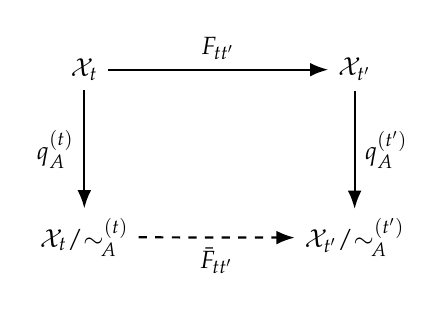
\begin{tikzpicture}[baseline=(current bounding box.center),
  node distance=2.4cm, every node/.style={font=\small}]
  \node (Xt)  {$\calX_t$};
  \node (Xtp) [right=2.8cm of Xt]  {$\calX_{t'}$};
  \node (Qt)  [below=1.5cm of Xt]  {$\calX_t/{\simA^{(t)}}$};
  \node (Qtp) [below=1.5cm of Xtp] {$\calX_{t'}/{\simA^{(t')}}$};
  \draw[-Latex,thick] (Xt)  -- node[above]{$F_{tt'}$} (Xtp);
  \draw[-Latex,thick] (Xt)  -- node[left]{$q_A^{(t)}$} (Qt);
  \draw[-Latex,thick] (Xtp) -- node[right]{$q_A^{(t')}$} (Qtp);
  \draw[-Latex,dashed,thick] (Qt) -- node[below]{$\bar{F}_{tt'}$} (Qtp);
\end{tikzpicture}
\end{equation}
commutes, where $\bar{F}_{tt'}$ is the map on quotients induced by $F_{tt'}$
via the universal property of $q_A^{(t')}$.
\end{theorem}

\begin{proof}
The commutativity of~\eqref{eq:meta} is equivalent to $q_A^{(t')} \circ
F_{tt'} = \bar{F}_{tt'} \circ q_A^{(t)}$. The map $\bar{F}_{tt'}$ exists
by the universal property (Theorem~\ref{thm:universal}) iff $q_A^{(t')} \circ
F_{tt'}$ is strongly admissible from $(\calX_t, \simA^{(t)})$, which holds
iff $F_{tt'}$ is a morphism in $\Adm$: $x_1 \simA^{(t)} x_2 \Rightarrow
F_{tt'}(x_1) \simA^{(t')} F_{tt'}(x_2)$. The functoriality conditions then
follow from identity and composition in $\Adm$.
\end{proof}

\begin{corollary}[Closure Under Composition]
\label{cor:meta_compose}
If $F_{t,t+1}$ and $F_{t+1,t+2}$ are both admissibility-preserving, then
$F_{t,t+2} = F_{t+1,t+2} \circ F_{t,t+1}$ is admissibility-preserving.
Meta-admissibility is closed under composition.
\end{corollary}

\begin{proof}
Morphisms in $\Adm$ are closed under composition by Lemma~\ref{lem:category}.
\end{proof}

\begin{remark}[Non-morphisms Do Not Compose to Non-morphisms]
One might expect that a single inadmissible step should propagate forward,
``contaminating'' all subsequent admissibility structure. This expectation is
incorrect. In category theory, the composition of a non-morphism with a
morphism is in general neither a morphism nor a non-morphism in any systematic
way: a later transformation $F_{t+1,t+2}$ can re-separate states that
$F_{t,t+1}$ collapsed, thereby restoring admissibility at the composed level.
Formally, $f \notin \mathrm{Mor}(\Adm)$ does not imply $g \circ f \notin
\mathrm{Mor}(\Adm)$.

What is true is the contrapositive of Corollary~\ref{cor:meta_compose}: if the
composed transformation $F_{t,t+2}$ is not admissibility-preserving, then at
least one of $F_{t,t+1}$ or $F_{t+1,t+2}$ is not admissibility-preserving.
The diagnostic question is therefore: does the composed map fail to be a
morphism? If so, at least one step in the composition is inadmissible, though
which one (or ones) requires separate analysis.
\end{remark}

\subsection{Natural transformations between developmental trajectories}

\begin{definition}[Natural Transformation of Trajectories]
Two temporal admissibility functors $\mathbf{X}, \mathbf{Y}\colon
\mathbf{T} \to \Adm$ are compared by a \emph{natural transformation}
$\eta\colon \mathbf{X} \Rightarrow \mathbf{Y}$: a family of morphisms
$\eta_t\colon (\calX_t, \simA^X{}^{(t)}) \to (\calY_t, \simA^Y{}^{(t)})$
in $\Adm$ such that for all $t \leq t'$,
\[
  \eta_{t'} \circ F_{tt'}^X = F_{tt'}^Y \circ \eta_t.
\]
\end{definition}

A natural transformation $\eta$ between two trajectories is a time-indexed
family of admissibility-preserving maps between their state spaces that
commutes with temporal evolution in both trajectories. It provides a systematic
comparison of two developmental paths---two agents, or two stages of the same
agent under different conditions---that respects admissibility structure at
every time step.

%% =====================================================================
\section{The Admissibility Programme as a Geometric Object}
\label{sec:synthesis}
%% =====================================================================

The four structures developed in this paper fit together into a coherent
geometric picture of the admissibility programme.

At the level of a fixed state space $\calX$ with fixed policy class $\Pi$ and
horizon $H$: the admissibility quotient $q_A\colon \calX \to \XmodA$ is the
initial object in the category of strongly admissible projections
(Corollary~\ref{cor:initial}); every encoder $\varphi$ defines a point in
the quotient lattice $\calL(\calX)$, and admissibility distortion $\DA$ is a
monotone height function on this lattice increasing along compression morphisms
(Theorem~\ref{thm:monotone}); the global section $s^*\colon x \mapsto \RHP(x)$ of $\calF_A$ encodes
the complete reachability structure that planning requires; planning-adequate
representations are exactly those encoders $\varphi$ for which $\varphi(x_1)
\neq \varphi(x_2)$ whenever $s^*(x_1) \neq s^*(x_2)$---admissibility is
the condition that $\varphi$ separates the fibres of $s^*$---and
passive observation determines only local sections of $\calF_O$ over the
coarser topology $\tau_O$ (Theorem~\ref{thm:sheaf_oist}).

At the level of an evolving state space: temporal evolution is a functor
$\mathbf{X}\colon \mathbf{T} \to \Adm$ (Definition~\ref{def:temporal});
meta-admissibility is the condition that this functor exists with the required
commutativity (Theorem~\ref{thm:meta}); comparisons between developmental
trajectories are natural transformations between such functors.

The unifying geometric statement is:
\begin{quote}\itshape
Observation provides local sections of $\calF_O$ over the observation topology.
Planning requires a global section of $\calF_A$ over the reachability topology.
Admissibility distortion quantifies the obstruction to assembling the former
into the latter; Conjecture~\ref{conj:cohomology} proposes that this
obstruction is measured by the first \v{C}ech cohomology of $\calF_A$ with
respect to observational covers.
\end{quote}

This is the geometric form of the Observational--Interventional Separation
Theorem: not a logical implication between equivalence classes, but a failure
of the sheaf gluing axiom, measurable in principle by a cohomological invariant.
The admissibility programme---naming, estimating, and minimising $\DA$---is,
in this reading, the programme of computing, bounding, and eventually
eliminating a cohomological obstruction.

%% =====================================================================
\section{Open Problems}
\label{sec:open}
%% =====================================================================

\noindent\textbf{1. Proof of Conjecture~\ref{conj:cohomology}.} The central open
problem is to prove (or disprove) the cohomological admissibility obstruction
conjecture. The first step is a precise linearisation of $\calF_A$ as a sheaf
of abelian groups. The second is an explicit identification of the cohomology
class associated to admissibility distortion. The third is a norm on
$\check{H}^1(\mathcal{U}; \calF_A)$ with the required lower bound. Whether
the natural linearisation by indicator functions on $\calX \times \calX$
yields a tractable cohomology theory is the first technical question.

\medskip
\noindent\textbf{2. \v{C}ech cohomology of the reachability sheaf.} Even
independently of Conjecture~\ref{conj:cohomology}, the \v{C}ech cohomology
$\check{H}^*(\mathcal{U}; \calF_A)$ is a new mathematical object. Its
properties---whether higher cohomology groups are trivial, what covering
conditions minimise the first cohomology, how the cohomology changes under
changes in $\Pi$ and $H$---are largely unexplored. In particular, the
question of whether the reachability sheaf is acyclic (all higher cohomology
vanishing) would clarify the scope of obstructions.

\medskip
\noindent\textbf{3. Derived functors and the quotient sheaf.} If $\calF_A$ is
treated as a sheaf of abelian groups, the right-derived functors of the
global sections functor $\Gamma$ give sheaf cohomology groups $H^k(\calX,
\calF_A)$. Admissibility distortion may be recoverable as a specific class
in $H^1(\calX, \calF_A/\calF_O)$, the cohomology of the quotient sheaf. The
relationship between \v{C}ech cohomology and derived-functor cohomology in
this setting---which requires the reachability sheaf to satisfy an acyclicity
condition on the reachability topology---is a natural question.

\medskip
\noindent\textbf{4. The bisimulation tower.} Bisimulation equivalence is a
refinement of admissibility equivalence: $x_1 \sim_\mathrm{bis} x_2$ iff
the transition distributions are equal, which is a strictly stronger condition
than $\RHP(x_1) = \RHP(x_2)$. The bisimulation sheaf $\calF_\mathrm{bis}$
sits between $\calF_O$ and $\calF_A$ in a tower of sheaves over $\calX$.
The obstruction to lifting sections of $\calF_O$ to $\calF_\mathrm{bis}$ may
be computable in practice (since bisimulation metrics have efficient
approximations), providing a computable lower bound on the obstruction to
lifting to $\calF_A$.

\medskip
\noindent\textbf{5. Topos-theoretic internalisation.} The category $\Adm$
with the Alexandrov topology on each object suggests a site $(\Adm, \tau_A)$
obtained by equipping $\Adm$ with a Grothendieck topology. The topos of
sheaves $\mathbf{Sh}(\Adm, \tau_A)$ would provide a generalised geometric
universe in which admissibility arguments can be conducted internally. Whether
the internal logic of this topos has a natural interpretation in terms of
planning-theoretic reasoning---and in particular, whether the universal
property of $q_A$ has a clean internal formulation---is an open question. The
definition of the Grothendieck topology on $\Adm$ itself (as opposed to on
individual objects) requires separate development.

\medskip
\noindent\textbf{6. Persistent homology of reachability.} For metric state
spaces with $\calX \subseteq \R^n$, the reachability sets $\RHP(x)$ vary
with $x$. The filtration
\[
  \bigl\{\mathcal{R}_h^\Pi(x)\bigr\}_{h = 0}^{H}
\]
of reachability sets as the horizon $h$ grows from $0$ to $H$ defines a
filtered topological space for each $x$. The persistent homology of this
filtration captures how topological features of the reachability geometry
appear and disappear as the planning horizon grows. The birth and death times
of homological features are intrinsic invariants of the policy class $\Pi$
and may provide a topological analogue of admissibility depth.

\medskip
\noindent\textbf{7. Enriched and $(\infty,1)$-categorical generalisations.}
The category $\Adm$ as defined is an ordinary category. Two natural enrichments
are worth exploring: an \emph{enrichment over metric spaces} (with the
admissibility distortion $\DA$ as a distance between morphisms) and an
\emph{$(\infty,1)$-categorical} version (replacing sets of morphisms by
spaces of morphisms, with higher morphisms encoding homotopies of
admissibility-preserving maps). The latter would connect the admissibility
programme to the emerging theory of reachability in homotopy type theory.

%% =====================================================================
\section{Conclusion}
\label{sec:conclusion}
%% =====================================================================

We have developed the geometry of admissibility through four interlocking
structures. The category $\Adm$ provides the natural language for speaking
about admissibility-preserving maps: admissible representations are morphisms,
the admissibility quotient is an initial object with a universal property, and
admissibility distortion measures deviation from morphismhood. The quotient
lattice organises all possible compressions of a state space into a partial
order on which distortion is monotone, making the compression--admissibility
tradeoff a functor. The reachability sheaf over the Alexandrov topology shows
that planning requires global sections and observation provides only local
ones, with the separation between the two sheaves being a failure of sheaf
gluing. Temporal admissibility functors capture evolving state spaces and
characterise meta-admissibility as the functor condition.

The central mathematical object that emerges is the reachability sheaf $\calF_A$
over the Alexandrov topology $\tau_A$. Its canonical global section $s^*\colon
x \mapsto \calR^\Pi(x)$ encodes the complete reachability structure. A
representation $\varphi\colon \calX \to \calM$ is planning-adequate precisely
when it separates the fibres of $s^*$: admissibility is the condition
$s^*(x_1) \neq s^*(x_2) \Rightarrow \varphi(x_1) \neq \varphi(x_2)$. The distance from the observation sheaf
$\calF_O$ to the reachability sheaf is the geometric form of the
Observational--Interventional Separation Theorem. The quantitative measure of
this distance, which we conjecture to be the first \v{C}ech cohomology class
of $\calF_A$ relative to observational covers, is admissibility distortion.
The admissibility programme---developing estimators for $\DA$, designing
admissible encoders, characterising the information-theoretic constraints on
planning---is, in this geometric reading, the programme of computing, bounding,
and eventually eliminating a cohomological obstruction.

\bigskip
\noindent\textbf{Acknowledgements.} The author has no institutional affiliation
and no conflicts of interest.

\bigskip
\begin{thebibliography}{99}

\bibitem{kashiwara2006}
Kashiwara, M., and Schapira, P. (2006).
\textit{Categories and Sheaves}.
Springer.

\bibitem{maclane1998}
Mac~Lane, S. (1998).
\textit{Categories for the Working Mathematician}, 2nd ed.
Springer.

\bibitem{maclane1992}
Mac~Lane, S., and Moerdijk, I. (1992).
\textit{Sheaves in Geometry and Logic: A First Introduction to Topos Theory}.
Springer.

\bibitem{ferns2004}
Ferns, N., Panangaden, P., and Precup, D. (2004).
Metrics for finite Markov decision processes.
\textit{Proceedings of the Twentieth Conference on Uncertainty in
Artificial Intelligence (UAI)}, 162--169.

\bibitem{pearl2009}
Pearl, J. (2009).
\textit{Causality: Models, Reasoning, and Inference}, 2nd ed.
Cambridge University Press.

\bibitem{quillen1967}
Quillen, D. (1967).
\textit{Homotopical Algebra}.
Lecture Notes in Mathematics, vol.\ 43.
Springer.

\bibitem{bredon1997}
Bredon, G. E. (1997).
\textit{Sheaf Theory}, 2nd ed.
Graduate Texts in Mathematics, vol.\ 170.
Springer.

\bibitem{grothendieck1957}
Grothendieck, A. (1957).
Sur quelques points d'alg\`ebre homologique.
\textit{T\^ohoku Mathematical Journal}, 9(2), 119--221.

\bibitem{chen2026}
Chen, Z., Wang, Y., Bai, Y., et al. (2026).
MAE-YOLO improves small object detection for intelligent inspection.
\textit{Scientific Reports}.

\bibitem{mueller2026}
Mueller, T.T., Starck, S., Llalloshi, R., et al. (2026).
Local and global patterns support medical imaging as a biomarker of ageing.
\textit{Communications Medicine}, 6, 335.

\bibitem{zhang2026}
Zhang, J., Deng, Z., Li, X., et al. (2026).
Enhanced human pose estimation via self-distilled and token-pruned transformer.
\textit{Scientific Reports}.

\end{thebibliography}

\end{document}
